
\subsection{Comportamientos e implementaciones}
\label{comportamientos}

Una vez que decidimos utilizar la arquitectura explicada en la secci\'on
\ref{arq_prop} para nuestro proyecto, tuvimos que analizar:
\begin{itemize}
\item{}Forma de implementaci\'on de la arquitectura en c\'odigo,
\item{}Comportamientos a realizar,
\item{}Ordenes de inhibici\'on y supresi\'on entre los mismos,
\item{}Forma de implementaci\'on de los mismos,
\item{}Orden de implementaci\'on
\end{itemize}

%Detallar que se hizo con cada item
Para implementar la arquitectura decidimos asignarle un $ID$ num\'erico
diferente a cada comportamiento. Tambi\'en tomamos la decisi\'on de elegir como
comportamiento activo en el instante $t$, aquel comportamiento que est\'e
activo en ese instante y tenga mayor $ID$, suprimiendo as\'i el resto de los
comportamientos (con un $ID$ menor) que podr\'ian estar activos.

%Explicar como se relaciona el requerimiento (robot recolector de basura
%autonomo) con los comportamientos que pusimos
Como requerimiento de nuestro proyecto ten\'iamos la realizaci\'on de un robot
aut\'onomo que recolecte basura de su entorno din\'amico pero estructuralmente
est\'atico. De aqu\'i se infieren algunos de los comportamientos que debe tener
el robot:
\begin{itemize}
	\item{\emph{Recolectar basura} (\ref{collect_garbage})}
	\item{\emph{Recargar bater\'ia} (\ref{recharge_battery}):} Por ser
		aut\'onomo, debe poder ser capaz de recargarse solo para poder continuar
		con su actividad.
	\item{\emph{Wandering} (\ref{wandering}):} El robot, al ser aut\'onomo, no es
		radio-controlado y debe poder recorrer el entorno por s\'i mismo.
	\item{\emph{Evitamiento de obst\'aculos} (\ref{avoid_obstacles}):} Debido a
		la naturaleza din\'amica del entorno, el robot debe ser capaz de navegar
		sin chocarse contra las paredes ni con las personas que circulan por
		el mismo.
\end{itemize}

El comportamiento de recolectar basura y el requerimiento de la autonom\'ia
llevan a su vez a la aparici\'on de m\'as comportamientos: \emph{Descargar
basura} (\ref{unload_garbage}) e \emph{Ir hacia basura} (\ref{go_to_garbage}).
\\\indent
En la figura \ref{fig:architecture} mostramos los comportamientos implementados
y su orden de jerarqu\'ia. Se puede ver que hay m\'as comportamientos de los
detallados anteriormente ya que la forma en que implementamos los
comportamientos b\'asicos del robot requiri\'o el desarrollo de otros
auxiliares.
\\\indent
\begin{figure}[htp]
\begin{center}
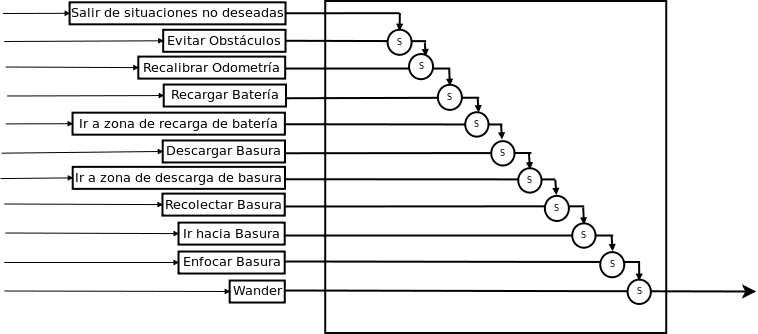
\includegraphics[scale=0.5]{comportamientos/figures/behavioursArchitecture2.png}
\caption{Arquitectura de comportamientos implementada}
\label{fig:architecture}
\end{center}
\end{figure}
\\\indent
Primero implementamos \emph{Wandering} debido, en una primera aproximaci\'on,
a su sencillez. Luego implementamos \emph{Evitamiento de obst\'aculos}
para lograr que el robot pueda navegar sin problemas por el entorno. Como el
comportamiento de recolectar e ir hacia la basura dependend\'ia del m\'odulo
de reconocimiento de objetos y el mismo estaba siendo desarrollado en paralelo,
decidimos implementar el comportamiento de \emph{Recargar bater\'ia} y
\emph{Descargar basura}. Una vez que tuvimos la primera implementaci\'on
funcional del reconomiento de objetos, procedimos a desarrollar
\emph{Ir hacia basura} y \emph{Recolectar Basura}.
\\\indent
A continuaci\'on detallamos los comportamientos indicados en la figura
\ref{fig:architecture}, as\'i como su implementaci\'on en 
\emph{pseudo-c\'odigo} y detalles tenidos en cuenta para su realizaci\'on.
%A continuacion vamos a explicar cada comportamiento.....

\subsubsection{Wandering}
\label{wandering}

\paragraph{Detalle del comportamiento} 
Por ser el comportamiento que menor jerarqu\'ia tiene (Ver figura
\ref{fig:architecture}), es el \'unico comportamiento que est\'a activo
ante la ausencia de un est\'imulo, asegurandonos que siempre haya por lo menos
un comportamiento activo.
\\\indent
En una primera aproximaci\'on de \emph{Wandering}, s\'olo nos preocupamos por
ir hacia adelante ya que eventualmente, el robot encuentra un obst\'aculo y
realiza un giro cambiando su direcci\'on.
\\\indent
Los resultados de la simulaci\'on nos indicaron que el robot no recorr\'ia
ciertas zonas o las recorr\'ia despu\'es de un largo tiempo, lo que nos llev\'o
a una segunda implementaci\'on. La misma lleva un seguimiento de los
lugares que m\'as recientemente recorri\'o el robot. Adem\'as, hicimos uso de la
c\'amara para redefinir la idea de zona recorrida. Decimos que el robot
recorri\'o cierta zona si:
\begin{itemize}
	\item{}Estuvo f\'isicamente en ella, o
	\item{}La zona fue alcanzada por la imagen que se ve en la c\'amara
			(Ver figura \ref{fig:zoneCamera})
\end{itemize}
\'Esto, en cierta forma, genera un modelo del mundo, un hecho que
conflict\'ua con uno de los principios propuestos a seguir en la secci\'on
\ref{arq_prop}. Para minimizar el conflicto, decidimos mantener al m\'inimo la
informaci\'on almacenada para el funcionamiento del algoritmo, es decir, por
cada zona de la arena s\'olo mantenemos el timestamp de la \'ultima vez que el
robot la visit\'o.

\paragraph{Implementaci\'on del comportamiento}

La segunda implementaci\'on en \emph{pseudo-c\'odigo} es la siguiente:
\begin{verbatim}
por cada paso
    zona = pedir_zona_vista(camara)
    marcar_zona_como_vista(modelo_del_mundo,zona)
    ultima_zona_visitada = pedir_ultima_zona_visitada(modelo_del_mundo)
    velocidades = calcular_velocidades_de_ruedas(ultima_zona_visitada)
    poner_velocidades_en_ruedas(velocidades)
\end{verbatim}
Para obtener la zona vista por la c\'amara, necesitamos de la altura $C_h$ a la
cual est\'a ubicada la c\'amara en el robot, el campo de visi\'on (de ahora en
adelante \emph{Field of View o FOV}) horizontal $FOV_h$ o vertical $FOV_v$ y
el \'angulo de inclinaci\'on de la c\'amara $ac$. Analizando la figura 
\ref{fig:angleCamera} podemos ver que:

\begin{figure}[htp]
\begin{center}
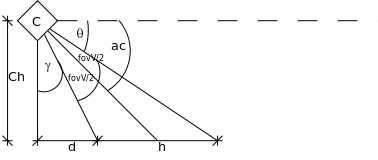
\includegraphics{comportamientos/figures/angleCamera.png}
\caption{Diagrama de posici\'on de la c\'amara}
\label{fig:angleCamera}
\end{center}
\end{figure}

\begin{eqnarray}
ac = \frac{FOV_v}{2} + \theta\\
\gamma + FOV_v + \theta = \frac{\pi}{2}\\
\tan(\gamma) = \frac{d}{C_h}\\
\tan(\gamma+FOV_v) = \frac{d+h}{C_h}
\end{eqnarray}

%En caso de no disponer del $FOV_v$, el mismo se puede obtener de:
%\begin{equation}
%FOV_v = \atan(\frac{ \tan(\frac{FOV_h}{2}) * height}{width} * 2)\\
%\end{equation}
Organizando las ecuaciones, podemos deducir que:

\begin{eqnarray}
\gamma = \frac{\pi}{2} + ac - \frac{FOV_v}{2}\\
\label{eqn:distance_d}
d = \tan(\gamma) * C_h \\
\label{eqn:distance_dh}
d+h = \tan(\gamma+FOV_v) * C_h
\label{wander:ecfov}
\end{eqnarray}

Por lo que obtenemos el \'angulo hasta el inicio de la im\'agen de la c\'amara
$\gamma$ y como consecuencia, la distancia $d$ desde la posici\'on de la
c\'amara hasta el inicio de la im\'agen y $d+h$, la distancia desde la
posici\'on de la c\'amara hasta el final de la im\'agen. Usando estos datos,
la posici\'on del robot $P$ y bas\'andonos en la figura \ref{fig:zoneCamera},
podemos obtener los puntos $A$, $B$, $C$ y $D$ del trapezoide que determina la
zona que ve la c\'amara.

\begin{figure}[htp]
\begin{center}
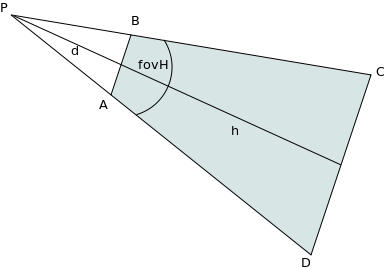
\includegraphics[scale=0.5]{comportamientos/figures/rectangleWander.png}
\caption{Zona vista por la c\'amara}
\label{fig:zoneCamera}
\end{center}
\end{figure}

\subsubsection{Enfocar Basura}
\label{focus_garbage}
Una vez que el m\'odulo de detecci\'on de objetos reconoce algo como basura
(ver secci\'on \ref{algoritmo_vision}), hay que elegir
la forma en que se va a la basura. En la figura \ref{fig:papproachgoto}
mostramos una aproximaci\'on. Consiste en primero enfocar la
basura de forma tal que la misma quede en el centro de la imagen de la
c\'amara. De aqu\'i surge el comportamiento \emph{Enfocar Basura}.
\\\indent
Una segunda forma de lograr \'esto (figura \ref{fig:sapproachgoto}) no consiste
en enfocar la basura, sino que se marca un arco hacia la misma. \'Esto requiere
que se seteen las velocidades correspondientes a las ruedas de forma tal que la
trayectoria del robot describa dicho arco. Con esta alternativa no
existir\'ia el comportamiento que se est\'a describiendo.
\\\indent
Dado que la primera aproximaci\'on es levemente m\'as simple de implementar, y
teniendo en cuenta el principio enunciado en la secci\'on \ref{arq_prop}
\emph{``La simplicidad es una virtud''}, elegimos implementarlo, a
pesar de tener un posible inconveniente, como mostramos en la figura
\ref{fig:papproachgotoproblem}.
\\\indent
Cuando hay una basura en alguna esquina superior de la imagen de la c\'amara,
y el robot gira sobre s\'i mismo para enfocarla, la basura puede llegar a
perderse por el fondo de la imagen. \'Esto se debe a que la distancia hacia
dichas esquinas es mayor a la distancia hacia el centro del borde superior de
la imagen (ver figura \ref{fig:zoneCamera}). Decimos que es un ``posible''
problema, ya que una vez que se pierde de vista la basura, el robot no
enfocar\'a m\'as debido a que el est\'imulo desapareci\'o, pero si luego se
dirige hacia adelante (por la activaci\'on de alg\'un otro comportamiento), la
basura volver\'a a aparecer en la imagen, sin desaprovechar la oportunidad de
recogerla.

\begin{figure}[htp]
\begin{center}
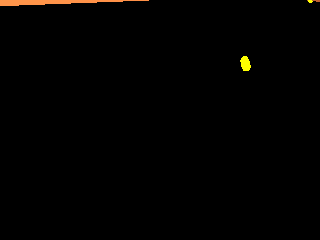
\includegraphics[scale=0.5]{comportamientos/figures/basura.png}
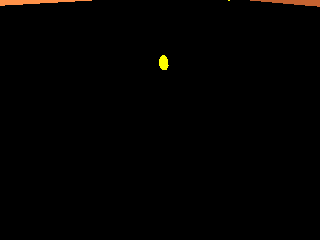
\includegraphics[scale=0.5]{comportamientos/figures/basuraenfocada.png}
\caption[Primera aproximaci\'on de ``Ir a la basura'']{Primera aproximaci\'on
		de ``Ir a la basura''. Inicialmente el objeto
		reconocido como basura se encuentra a un costado del eje vertical de
		la imagen. Luego el robot gira de forma tal que el objeto quede sobre
		el eje vertical.}
\label{fig:papproachgoto}
\end{center}
\end{figure}

\begin{figure}[htp]
\begin{center}
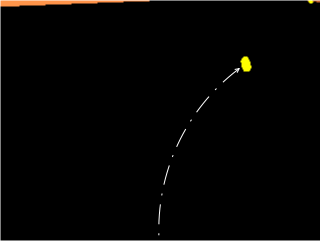
\includegraphics[scale=0.5]{comportamientos/figures/basuraAlt.png}
\caption[Segunda aproximaci\'on de ``Ir a la basura'']{Segunda aproximaci\'on de ``Ir a la basura''. Se traza un arco hacia
		el objetivo de forma tal que no sea necesario enfocar la basura.}
\label{fig:sapproachgoto}
\end{center}
\end{figure}

\begin{figure}[htp]
\begin{center}
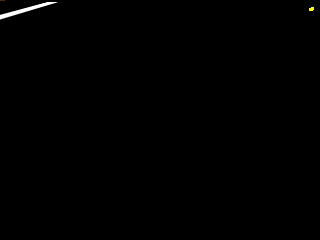
\includegraphics[scale=0.3]{comportamientos/figures/esquina.png}
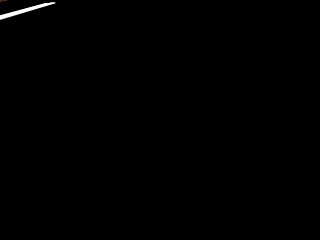
\includegraphics[scale=0.3]{comportamientos/figures/frentemuylejos.png}
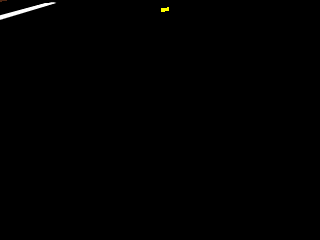
\includegraphics[scale=0.3]{comportamientos/figures/frentelejos.png}
\caption[Inconveniente con la primera aproximac\'ion de
		``Ir a la basura'']{Posible inconveniente con la primera aproximac\'ion
		de ``Ir a la basura''. La basura se encuentra en una de las
		esquinas superiores de la im\'agen. El robot la enfoca, girando
		hacia la derecha y la basura desaparece de la imagen. En el caso
		que el robot se dirija hacia adelante, la basura volver\'a a
		aparecer en la im\'agen.}
\label{fig:papproachgotoproblem}
\end{center}
\end{figure}

\paragraph{Detalle del comportamiento}
La primer aproximaci\'on se puede describir como:
\begin{itemize}
\item Si la basura est\'a a la izquierda de la im\'agen, se debe girar hacia la
			izquierda
\item Si la basura est\'a a la derecha de la im\'agen, se debe girar hacia la
			derecha
\item Si la basura est\'a en el centro, ya est\'a enfocada
\end{itemize}

%En el caso que haya m\'as de una basura elegimos la m\'as cercana, usando
%c\'alculos detallados a continuaci\'on.
\paragraph{Implementaci\'on del comportamiento}
\label{focus_garbage:impl}
Para la implementaci\'on se sigue el siguiente \emph{pseudo-c\'odigo}:
\begin{verbatim}
por cada paso
    lista_de_basuras = obtener_lista_de_basuras(modulo_de_reconocimiento)
    basura_mas_cercana = elijo_basura_mas_cercana(lista_de_basuras)
    angulo_a_basura = obtener_angulo(basura_mas_cercana)
    velocidad = VELOCIDAD_BASE * (abs(angulo_a_basura) / (PI/2))
               + VELOCIDAD_BASE_MINIMA

    si angulo_a_basura < 0 entonces
        veloc_izq = -velocidad
        veloc_der = velocidad
    sino
        veloc_izq = velocidad
        veloc_der = -velocidad
    fin_si
    poner_velocidades_en_ruedas(veloc_izq, veloc_der)
\end{verbatim}


Se puede ver que la velocidad de giro del robot es proporcional al m\'odulo del
\'angulo que hay hacia la basura, logrando enfocar m\'as r\'apido cuando el
\'angulo es mayor y tener mayor precisi\'on cuando el \'angulo es m\'as chico,
adem\'as de tener mayor rapidez de enfoque y precisi\'on que si la velocidad de
giro fuera constante.
\\\indent Como observamos en el pseudo-c\'odigo del cuadro \ref{focus_garbage:impl},
el algoritmo selecciona, la basura que se encuentra mas cercana 
al robot. Para esto realiza una transformaci\'on en la cual obtiene la distancia al objeto seg\'un
su coordenada $(x,y)$ en la imagen. Observando la figura \ref{fig:altoDiag} apreciamos que 
la distancia a un objeto $r$ puede calcularse mediante la siguiente ecuaci\'on:
\begin{equation}
r=\sqrt{a^2 + c^2}
\label{eq:posta}
\end{equation}
Los valores de $a$ y $c$ no son conocidos. Comenzando con $a$, si observamos la
figura \ref{fig:trianglesAB} podemos afirmar que:
\begin{equation}
a=2b \sin(\frac{\alpha}{2})
\label{eq:asin}
\end{equation}
donde $b$, a su vez, lo calculamos como:
\begin{equation}
b=\sqrt{c^2+ Ch^2}
\label{eq:depc}
\end{equation}
$Ch$ representa la altura de la c\'amara y es un valor conocido.\\
\indent Sin embargo para el calculo de $c$ tenemos que recurrir a la ecuaci\'on 
\ref{wander:ecfov} donde reemplazamos $FOV_v$ por $\beta$ que es el \'angulo que forma la 
c\'amara con el objeto en cuesti\'on. \'Este se computa como $\beta=k FOV_v$ donde $k=dist_y / RES_h$ que se corresponden con 
la distancia en pixels sobre el eje $y$ y la resoluci\'on horizontal de la imagen respectivamente. El calculo de $k$ puede apreciarse 
mejor en la figura \ref{fig:image_coord_conv}.\\ Para el computo de la ecuaci\'on \ref{eq:asin} tambi\'en es necesario el 
valor de $\alpha$ el cual lo computamos como $\alpha=kp FOV_h / 2$ donde en este caso $kp$ y $FOV_h$ se corresponden con 
la distancia en pixeles sobre el eje $x$ y la resoluci\'on horizontal de la imagen. Habiendo obtenido estos valores, estamos en
condiciones de calcular tanto la ecuaci\'on \ref{eq:depc} como \ref{eq:asin} y finalmente, utilizando estos resultados, 
reemplazamos en \ref{eq:posta} y obtenemos la distancia hacia el objeto.

\begin{figure}[htp]
\begin{center}
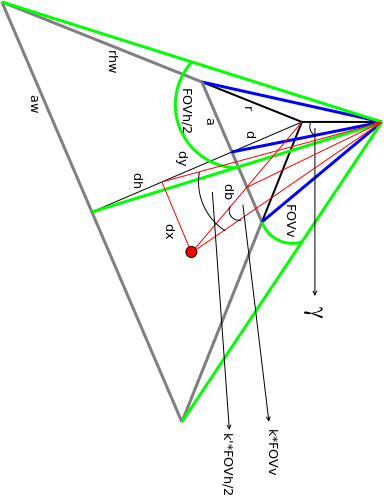
\includegraphics[scale=0.5]{comportamientos/figures/altoDiagram.png}
\caption[GUILLE COMPLETAR]{GUILLE COMPLETAR.}
\label{fig:altoDiag}
\end{center}
\end{figure}

\begin{figure}[htp]
\begin{center}
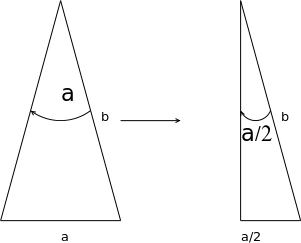
\includegraphics[scale=0.5]{comportamientos/figures/trianglesAB.png}
\caption[GUILLE COMPLETAR]{GUILLE COMPLETAR.}
\label{fig:trianglesAB}
\end{center}
\end{figure}


%%Para obtener el \'angulo y distancia hacia una basura....
%%pasamos de una posicion (x,y) en la imagen a una posicion
%(x,z) en el mundo. teniendo nuestra posicion P, podemos
%calcular la distancia y el angulo
\subsubsection{Ir a Basura}
\label{go_to_garbage}
Luego de la elecci\'on de la forma en que se resuelve el problema de encontrar
una basura (ver figura \ref{focus_garbage}), el comportamiento de ir a basura
resulta trivial, ya que luego de ser enfocada, la basura est\'a delante del
robot y lo basta con ir hacia adelante.

\paragraph{Detalle del comportamiento}
El est\'imulo necesario para que este comportamiento est\'e presente, est\'a
dado por dos condiciones:
\begin{enumerate}
\item El m\'etodo de reconocimiento de objetos encontr\'o una basura
\item La basura se encuentra en un entorno del centro del eje vertical de la
		im\'agen obtenida de la c\'amara.
\end{enumerate}
Para decidir si una basura se encuentra en un entorno del eje vertical,
utilizamos un umbral $\delta_f$ que determina el \'angulo de abertura.
Si una basura se encuentra en la zona, entonces se la toma como enfocada.
En la figura \ref{fig:focusAngles} se pueden ver 2 valores distintos para el
umbral.
\begin{figure}[htp]
\begin{center}
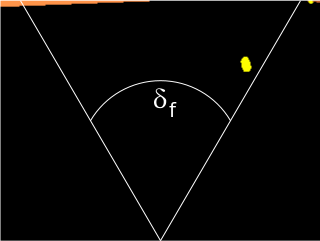
\includegraphics[scale=0.5]{comportamientos/figures/garbageFocusAngle.png}
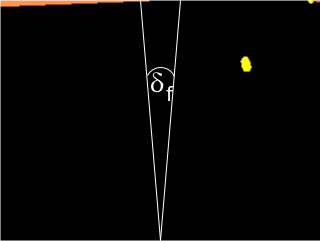
\includegraphics[scale=0.5]{comportamientos/figures/garbageFocusAngleTwo.png}
\caption{Distintos $\delta_f$}
\label{fig:focusAngles}
\end{center}
\end{figure}

\paragraph{Implementaci\'on del comportamiento}
\label{go_to_garbage:impl}
\begin{verbatim}
por cada paso
    distancia = obtener_distancia_a_basura(modulo_de_reconocimiento)
    coeff = (distancia - DIST_MIN)/(DIST_MAX - DIST_MIN)
    veloc_der = VELOCIDAD_MIN*(1 - coeff) + coeff*VELOCIDAD_MAX
    veloc_izq = veloc_der
    poner_velocidades_en_ruedas(veloc_izq, veloc_der)
\end{verbatim}

Al igual que en la implementaci\'on del comportamiento \ref{focus_garbage:impl},
las velocidades que se le otorgan a las ruedas dependen de la distancia
hacia la basura, de forma tal que si una basura est\'a muy lejos, la velocidad
sea mayor y a medida que se va acercando, vaya disminuyendo linealmente.

Dado que la basura se encuentra en un entorno del eje Y en la imagen (Ver figura
\ref{fig:image_coord_conv}b) cometemos un error muy peque\~no al estimar la
distancia a la basura como si estuviera sobre el mismo (asumiendo que la
coordenada X de la basura en la imagen es 0).

Como mostramos en las figuras \ref{fig:image_coord_conv} y
\ref{fig:angleCamera}, el \'angulo vertical hacia el punto m\'as alto de la
imagen $(0$,$C_{rh})$ es $\gamma+FOV_v$ y hacia el m\'as bajo, $(0$,$0)$, el
\'angulo es $\gamma$. De las ecuaciones \eqref{eqn:distance_d} y
\eqref{eqn:distance_dh} sabemos las distancias a los puntos $(0$,$0)$ y
$(0$,$C_{rh})$ son (DIST\_MIN) y (DIST\_MAX) respectivamente.
Entonces, para obtener la distancia $dy$ hacia el punto $(0$,$y)$ basta con
calcular:
\begin{eqnarray}
y_{angle} = FOV_v * \frac{y}{h} \\
dy = \tan(\gamma + y_{angle}) * C_h
\end{eqnarray}

donde $y_{angle}$ es la proporci\'on de $FOV_v$ hacia $y$.
\begin{figure}[htp]
\begin{center}
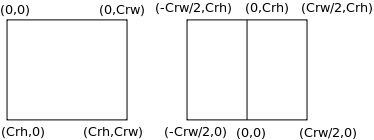
\includegraphics[scale=0.5]{comportamientos/figures/imageCoordsConvertion.png}
\caption[Conversi\'on de coordenadas de imagen de c\'amara]{Conversi\'on de
		coordenadas de imagen de c\'amara. Dado un pixel ($y$,$x$), su nueva
		coordenada est\'a dada por ($x-Crw/2$,$Crh-y$)}
\label{fig:image_coord_conv}
\end{center}
\end{figure}

\subsubsection{Recolectar Basura}
\label{collect_garbage}
Una vez que el robot lleg\'o a estar posicionado para recolectar la basura
deseada, el comportamiento de \emph{recolectar basura} se activa. El mecanismo
para lograr \'esto fue cambiando a lo largo del desarrollo del proyecto.
\\\indent
En un principio pensamos en usar una rampa interna dentro del robot, de forma
tal que la basura suba esa rampa para luego caer en un dep\'osito interno.
Por problemas con la simulaci\'on de este procedimiento, buscamos otro
mecanismo.
\\\indent
El mecanismo que elegimos para usar en la simulaci\'on tiene estas componentes:
\begin{itemize}
	\item El robot tiene un servo en su parte posterior (debajo de la c\'amara)
	\item Dos paredes delimitan el espacio a lo largo de la direcci\'on que une
			el centro del robot con el servo anteriormente mencionado.
\end{itemize}

\paragraph{Detalle del comportamiento}
La activaci\'on de \emph{recolectar basura} depende de 3 condiciones:
\begin{itemize}
	\item Las dos condiciones impuestas para \emph{ir a basura}
	\item La distancia a la basura elegida para ser recolectada debe ser menor a
			un umbral.
\end{itemize}

Aqu\'i se puede observar que tan importantes son los comportamientos anteriores
para que el robot logre recolectar la basura.
\\\indent
Es importante la elecci\'on del umbral: un valor muy chico, cercano a DIST\_MIN,
puede llevar a que el comportamiento no se active porque la basura ya no est\'a
m\'as en la imagen. Por otro lado, un valor muy grande, cercano a DIST\_MAX, 
causar\'ia que el robot se disponga a recolectar una basura que est\'a muy lejos
y podr\'ia llegar a moverse por cuestiones propias del ambiente, llevando as\'i
a una innecesaria activaci\'on del comportamiento.

\paragraph{Implementaci\'on del comportamiento}
El \emph{pseudo-c\'odigo} de este comportamiento es el siguiente:

\begin{verbatim}
    distancia = obtener_distancia_a_basura(modulo_de_reconocimiento)
    levantar(servo_delantero)
    recorrer_distancia(distancia)
    cerrar(servo_delantero)
\end{verbatim}

La distancia hacia la basura es obtenida de la misma forma que en la secci\'on
\ref{go_to_garbage:impl}. Levantar y cerrar el servo consiste en setear su
posici\'on en $\frac{\pi}{2}$ y $0$ respectivamente. Para calcular la distancia
recorrida utilizamos la distancia entre la posici\'on del robot en el
instante $t$, $P_r(t)$ y el instante $t+1$, $P_r(t+1)$, ambas dadas por la
odometr\'ia (Ver secci\'on \ref{odometry}). Las diferentes etapas de la
recolecci\'on de una basura las detallamos en la figura \ref{fig:recollection}.

\begin{figure}[htp]
\begin{center}
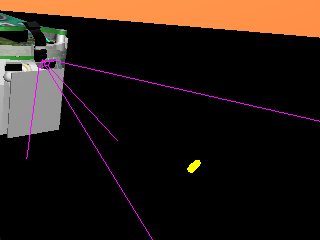
\includegraphics[scale=0.25]{comportamientos/figures/collect1.png}
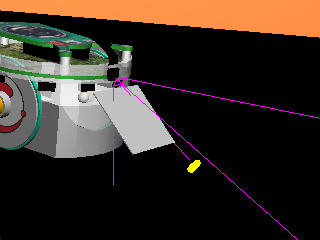
\includegraphics[scale=0.25]{comportamientos/figures/collect2.png}
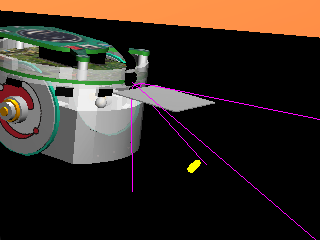
\includegraphics[scale=0.25]{comportamientos/figures/collect3.png}
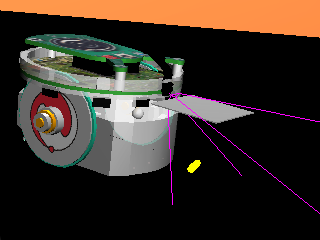
\includegraphics[scale=0.25]{comportamientos/figures/collect4.png}
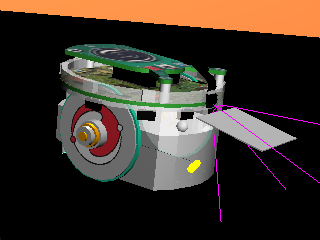
\includegraphics[scale=0.25]{comportamientos/figures/collect5.png}
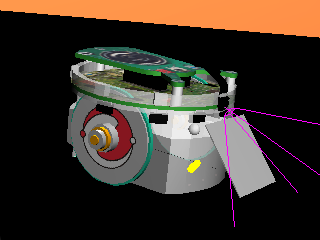
\includegraphics[scale=0.25]{comportamientos/figures/collect6.png}
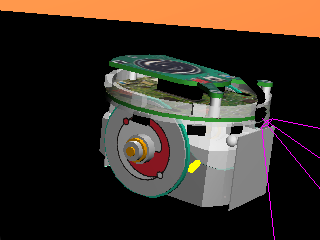
\includegraphics[scale=0.25]{comportamientos/figures/collect7.png}
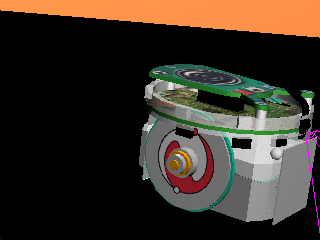
\includegraphics[scale=0.25]{comportamientos/figures/collect8.png}
%
\includegraphics[scale=0.3]{comportamientos/figures/unk.jpg}
\caption{Etapas de recolecci\'on de basura}
\label{fig:recollection}
\end{center}
\end{figure}


\subsubsection{Ir a zona de descarga de basura}
\label{go_to_unload_zone}
Como la capacidad del dep\'osito interno de basura del robot tiene un l\'imite, 
surge como necesidad que el robot sea capaz de ir hacia una zona donde
descargar\'a la basura que contiene. Entonces, al llenarse el dep\'osito
surge el est\'imulo necesario para la activaci\'on de este comportamiento.
\\\indent
Para ir hacia dicha zona decidimos imponerle una condici\'on al
entorno donde el robot actuar\'a. Esta condici\'on consiste en poner l\'ineas
de forma tal que si el robot la sigue, lo lleve a la zona de descarga.
\\\indent
Por lo tanto para dirigirse a la zona de descarga de basura, es necesario:
\begin{itemize}
	\item Buscar la l\'inea e ir a la misma
	\item Entrar a la l\'inea de forma tal que el robot y la l\'inea queden
				alineados
	\item Seguir la l\'inea
\end{itemize}
Siguiendo con la idea que es mejor descomponer un comportamiento complejo en
otros m\'as simples, decidimos separar el comportamiento de \emph{Ir a zona de
descarga de basura} en 3 comportamientos m\'as simples: \emph{Buscar l\'inea},
\emph{Entrar a la l\'inea} y finalmente \emph{Seguir la l\'inea}.

\paragraph{Buscar l\'inea}
\label{find_line}
Inicialmente hab\'iamos dispuesto las l\'ineas de forma tal que sigan los
l\'imites de la arena. Entonces para buscar la l\'inea tuvimos que calcular
para cada una cu\'al es la distancia hacia la misma, luego elegir ir a la
que menor distancia se encontraba. \'Esta implementaci\'on, adem\'as de ser
costosa, ten\'ia un problema: a veces suced\'ia que al ir hacia una l\'inea,
la distancia hacia otra pasaba a ser m\'as corta y \'esta \'ultima pod\'ia
estar m\'as lejos de la zona de recarga que la primera.
\\\indent
Luego repensamos el problema y nos dimos cuenta que el objetivo era llegar a la
zona de descarga, por lo que decidimos dejar s\'olo 2 las l\'ineas que se
encuentran a la misma distancia, como se puede apreciar en la figura
\ref{fig:arenafinal}. La zona de descarga se ubica cerca de donde se encuentra
el cilindro de color verde.
\\\indent
Para distinguir si el robot est\'a en una l\'inea o no, utilizamos sensores de
piso dispuestos como se muestra en la figura \ref{fig:floorSensors}. Los
sensores se encuentran a una distancia $Fsd$ del centro del robot sobre el eje
$Y$ y aquellos de los costados a una distancia $Fss$ del eje $Y$. La distancia
desde el sensor del medio hacia el centro del robot es $a$, mientras que la
distancia hacia un sensor del costado es $Fsl = \sqrt{Fsd^2 + Fss^2}$.

\begin{figure}[htp]
\begin{center}
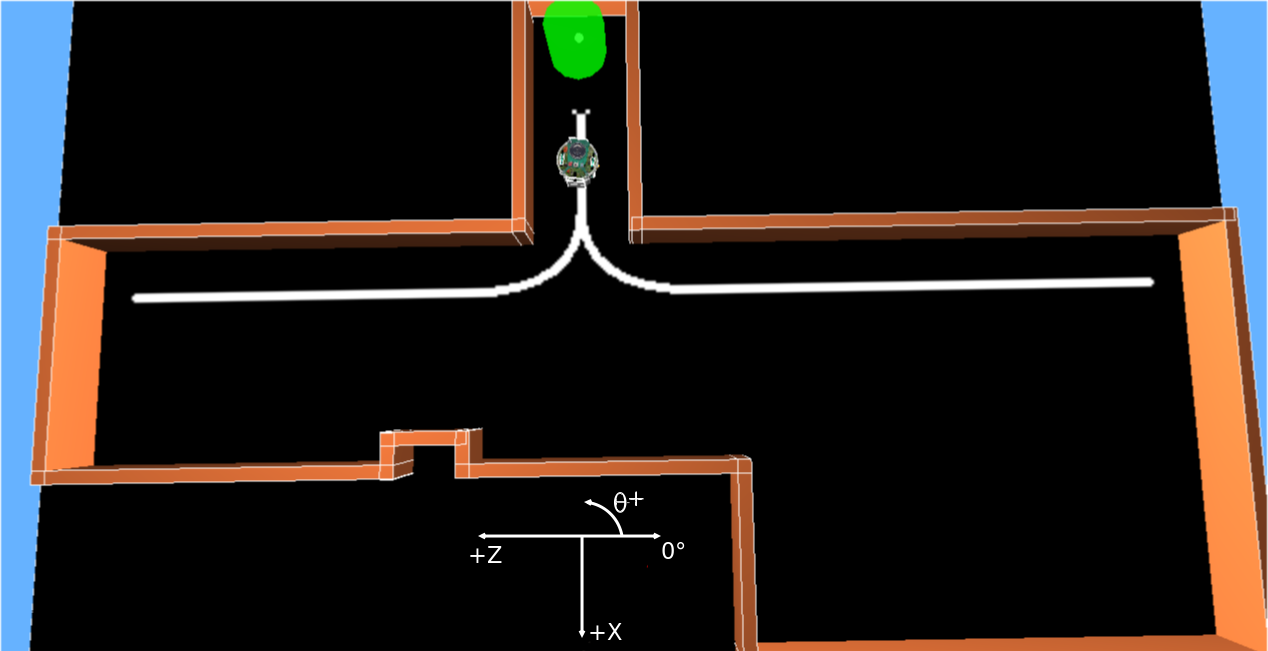
\includegraphics[scale=0.3]{comportamientos/figures/arenafinal.png}
\caption{Arena de simulaci\'on y ejes de coordenadas}
\label{fig:arenafinal}
\end{center}
\end{figure}

\begin{figure}[htp]
\begin{center}
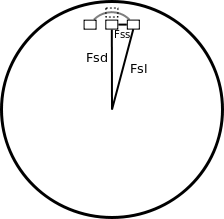
\includegraphics[scale=1.0]{comportamientos/figures/floorSensors.png}
\caption{Disposici\'on de sensores de piso}
\label{fig:floorSensors}
\end{center}
\end{figure}

\subparagraph{Detalle del comportamiento}
La decisi\'on de dejar s\'olo dos l\'ineas, acompa\~nada por la elecci\'on de
la ubicaci\'on de la zona de descarga, nos facilit\'o la composici\'on de
\'este comportamiento.
\\\indent Como mostramos en la figura \ref{fig:arenafinal}, para ir a la l\'inea se
debemos girar hasta tener un \'angulo de $\frac{\pi}{2}$ y luego ir hacia
adelante.

%Describir la eleccion de las distancias de las lineas hacia las paredes

\subparagraph{Implementaci\'on del comportamiento}
El \emph{pseudo-c\'odigo} de este comportamiento es sencillo, ya que
no requiere c\'alculos extras:

\begin{verbatim}
por cada paso
    angulo_actual = obtener_angulo_actual(odometria)
    si esta_en_un_entorno_de(angulo_actual, PI/2) entonces
        si angulo_actual > PI/2 && angulo_actual < 3PI/2 entonces
            giro_para_la_derecha
        sino
            giro_para_la_izquierda
        fin si
    sino
        voy_hacia_linea
    fin si
\end{verbatim}

Hicimos la verificaci\'on de que el \'angulo est\'e entre $\frac{\pi}{2}$ y
$\frac{3\pi}{2}$ para evitar girar m\'as de $\pi$, girando a la izquierda o a
la derecha dependiendo cual sea el caso. Para ver esto m\'as claramente,
veamos que sucediese si no estuviera:
\begin{verbatim}
    si esta_en_un_entorno_de(angulo_actual,PI/2) entonces
        giro_para_la_izquierda
    sino
\end{verbatim}
En el caso que el angulo actual sea $\pi$, el robot girar\'ia un total de
$\frac{3\pi}{2}$ hasta llegar al \'angulo destino $\frac{\pi}{2}$, cuando en
realidad girando para el sentido contrario s\'olo tendr\'ia que girar
$\frac{\pi}{2}$.
\\\indent
Se puede observar en el c\'odigo que usamos datos calculados por la
odometr\'ia, en este caso, la orientaci\'on actual del robot. El lector se
podr\'ia preguntar: ``Si la odometr\'ia tiene la posici\'on actual del robot,
?` porqu\'e no se usaron los datos de la misma para ir hacia la base?''. En
principio esto requiere que el robot tenga conocimiento acerca de la ubicaci\'on
de la base. Por otro lado, se hubiera tenido que utilizar alg\'un algoritmo de
\emph{Path Planning} para realizar el recorrido, algo que no concuerda con
la arquitectura elegida. Es importante destacar el uso de datos calculados por
la odometr\'ia porque si la misma llega a tener un error grande, puede llevar a
una activaci\'on err\'onea de comportamientos. Decimos que la odometr\'ia tiene
un error grande cuando, debido a esa magnitud, el robot no toma las decisiones
correctas debido al error en la informaci\'on en la cual se bas\'o. En la
secci\'on \ref{odometry:problems} se puede ver la incidencia de un error grande
de la odometr\'ia en el comportamiento emergente del robot.

\paragraph{Entrar a l\'inea}
\label{enter_line}
\subparagraph{Detalle del comportamiento}

Para seguir la l\'inea es necesario que primero el robot est\'e posicionado
sobre ella y alineado con la misma. Tambi\'en se necesita que la direcci\'on
del robot sea la que lo lleve hacia la zona de descarga. Una vez en
la l\'inea, el robot deber\'a girar dependiendo de que lado se encuentre la
misma (Ver figura \ref{fig:arenafinal}).

\subparagraph{Implementaci\'on del comportamiento}
\begin{verbatim}
    angulo_final = obtener_angulo_final(obtener_linea(odometria))
    tita = atan(dist_sens_piso_X, dist_sens_piso_Y)
    si (esta_en_la_linea(sensor_piso(DERECHA))) entonces
        tita = -tita
    fin si
    si (esta_en_la_linea(sensor_piso(MEDIO))) entonces
        tita = 0
    fin si
    si (tita != 0) entonces
        girar(tita)
    fin si
    distancia_a_recorrer = dist_sens_piso_Y;
    si (tita != 0) entonces
        distancia_a_recorrer = sqrt(dist_sens_piso_X^2 + dist_sens_piso_Y^2)
    fin si
    recorrer(distancia_a_recorrer)
    angulo_actual = obtener_angulo(odometria)
    girar(normalizar(angulo_actual - angulo_final))
\end{verbatim}

% Explicar el porque del primer giro
% Relacionarlo con la figura fig:floorSensors
El primer giro del robot es para lograr que el segmento que une el sensor de
piso del medio con el centro del robot quede ortogonal al segmento de l\'inea.
Como mostramos en la figura \ref{fig:floorSensorsInitialStates}, en el caso
(a) y (b) el robot girar\'a de forma tal que llegue un caso parecido al que
mostramos en la figura \ref{fig:floorSensorsFinalState} ya posiblemente el
sensor del medio no estar\'a en la l\'inea. Notar que si el sensor del medio
est\'a en la l\'inea, como es el caso de la figura
\ref{fig:floorSensorsInitialStates}c,
entonces el robot no gira, cualquiera sea el estado de los sensores de los
costados. El \'angulo que debe girar est\'a dado por $\theta = \arctan
(\frac{Fss}{Fsd})$ (Ver figura \ref{fig:floorSensors}) si debe girar hacia
la izquierda, o $-\theta$ en el otro caso.

\begin{figure}[htp]
\begin{center}
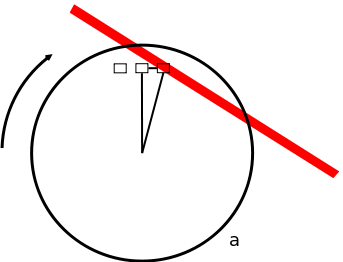
\includegraphics[scale=0.4]{comportamientos/figures/floorSensorsLine.png}
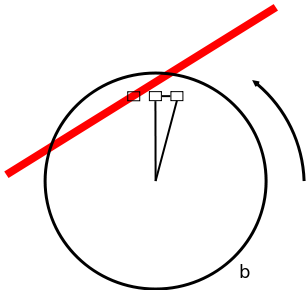
\includegraphics[scale=0.4]{comportamientos/figures/floorSensorsLine1.png}
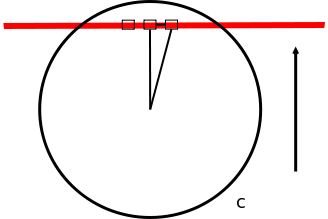
\includegraphics[scale=0.4]{comportamientos/figures/floorSensorsLine2.png}
\caption[Posibles estados iniciales de ``Entrar a la l\'inea'']{Posibles
		estados iniciales de ``Entrar a la l\'inea''. En el caso (a) el
		robot debe girar hacia la derecha. En el caso (b), el robot debe
		girar hacia la izquierda. En el caso (c) el robot no debe girar}
\label{fig:floorSensorsInitialStates}
\end{center}
\end{figure}

\begin{figure}[htp]
\begin{center}
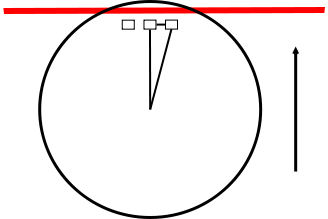
\includegraphics[scale=0.4]{comportamientos/figures/floorSensorsLine4.png}
\caption{Posible estado final luego del primer giro del comportamiento
		``Entrar a la l\'inea''}
\label{fig:floorSensorsFinalState}
\end{center}
\end{figure}

% Explicar el porque del recorrido de la distancia 
% Relacionarlo con la figura fig:floorSensors
Luego del posible giro para lograr que el sensor de piso del medio quede sobre
la l\'inea, se recorre una distancia de $Fsd$ en el caso que el robot no haya
girado anteriormente o $Fsl$ en el caso que s\'i lo haya hecho. El motivo de
realizar este trayecto es que el centro del robot quede sobre la l\'inea, como
muestra la figura \ref{fig:positioned}. De \'esta forma s\'olo queda girar
nuevamente hacia el \'angulo que se quiera. Si la l\'inea es la izquierda
entonces el robot deber\'a girar hasta que su orientaci\'on sea $0$ o $\pi$ en
el caso que la l\'inea sea la derecha.

\begin{figure}[htp]
\begin{center}
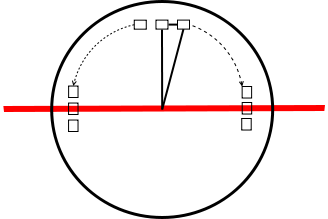
\includegraphics[scale=0.4]{comportamientos/figures/floorSensorsLine3.png}
\caption{Centro del robot sobre la l\'inea y posibles giros}
\label{fig:positioned}
\end{center}
\end{figure}

\paragraph{Seguir l\'inea}
\label{follow_line}
Una vez que el robot est\'a posicionado y con el sensor del medio sobre la
l\'inea, s\'olo basta con seguirla para llegar hacia la zona deseada. Este
comportamiento es sencillo de desarrollar.

\subparagraph{Detalle del comportamiento}
Para lograr que el robot siga la l\'inea debemos es tratar de mantener
s\'olo el sensor del medio sobre la l\'nea. Entonces, basta con analizar que se
debe hacer en los siguientes casos:
\begin{enumerate}
	\item El sensor de la derecha est\'a sobre la l\'inea
	\item El sensor de la izquierda est\'a sobre la l\'inea
\end{enumerate}
En el primer caso se debe lograr sacar el sensor de la derecha de la l\'inea
describiendo un peque\~no arco hacia ese lado. El segundo caso es an\'alogo:
para sacar el sensor de la izquierda de la l\'inea se debe seguir una
trayectoria con un peque\~no \'angulo hacia la izquierda. 

\subparagraph{Implementaci\'on del comportamiento}
El \emph{pseudo-c\'odigo} es simple:
\begin{verbatim}
por cada paso
    veloc_izq = veloc_der = VELOC_SEGUIR_LINEA
    si (esta_en_la_linea(sensor_piso(IZQUIERDA))) entonces
        veloc_izq *= (1 - FACTOR_DE_GIRO)
        veloc_der *= (1 + FACTOR_DE_GIRO)
    fin si
    si (esta_en_la_linea(sensor_piso(DERECHA))) entonces
        veloc_izq *= (1 + FACTOR_DE_GIRO)
        veloc_der *= (1 - FACTOR_DE_GIRO)
    fin si
    poner_velocidades_en_ruedas(veloc_izq, veloc_der)
\end{verbatim}

\subsubsection{Descargar Basura}
\label{unload_garbage}
Una vez que el robot logr\'o llegar a la zona de descarga de basura, debe
descargarla. Para hacer \'esto decidimos ubicar un servo en la parte trasera
del robot, con la misma idea del servo en el frente utilizado para
recolectar.

\paragraph{Detalle del comportamiento}
Para descargar la basura el robot debe posicionarse de forma tal que la
compuerta de descarga quede adyacente a la zona. Dado que para llegar a la
misma el robot sigui\'o la l\'inea, al finalizar va a estar orientado con un
\'angulo en un entorno de $\frac{\pi}{2}$ mirando la zona de descarga. Como el
servo de descarga se encuentra en la parte trasera, deber\'a realizar un giro
de aproximadamente $\pi$ para luego poder descargar la basura.
\paragraph{Implementaci\'on del comportamiento}
\begin{verbatim}
    posicionarse()
    levantar(servo_trasero)
    recorrerdistancia(ANCHO_ROBOT)
    cerrar(servo_trasero)
\end{verbatim}

\subsubsection{Ir a base de recarga de bater\'ia}
\label{go_to_recharge}
Ayudados por la elecci\'on que tomamos de poner la zona de descarga de basura
muy cercana a la zona donde se recarga la bater\'ia, decidimos utilizar la
misma estrategia de seguir la l\'inea para llegar hacia la misma.
\\\indent
La diferencia
entre ambos casos es el est\'imulo ante el cual se activan. En el caso de
ir a la zona de descarga, el est\'imulo proviene del sensor del dep\'osito
interno de basura que indica que el mismo est\'a lleno. En el caso de ir
a la base de recarga de bater\'ia, el est\'imulo para la activaci\'on depende
de los valores de dos sensores de bater\'ia que indican bater\'ia baja:
\begin{itemize}
	\item El sensor de la bater\'ia del robot, de donde se alimentan los sensores,
			actuadores y motores.
	\item El sensor de la computadora que corre el controlador.
\end{itemize}

\subsubsection{Cargar Bater\'ia}
\label{recharge_battery}
\paragraph{Detalle del comportamiento}
Una vez que el robot logr\'o llegar a la zona de recarga de bater\'ia, debe
recargarse. Para \'esto, debe posicionarse para lograr ubicarse el cargador
y esperar hasta que la bater\'ia alcance un valor de carga tal que le
permita seguir buscando basura sin problemas de bater\'ia.

\paragraph{Implementaci\'on del comportamiento}
\begin{verbatim}
    posicionarse()
    mientras(bateria_no_llena(BATERIA_ROBOT)
            o bateria_no_llena(BATERIA_PC)) hacer

        esperar(time_step)
    fin mientras
\end{verbatim}

\begin{comment}

\subsubsection{Recalibrarse}
\label{recalibrate}
\paragraph{Detalle del comportamiento}
\paragraph{Implementaci\'on del comportamiento}

\end{comment}

\subsubsection{Evitar Obst\'aculos}
\label{avoid_obstacles}
\emph{Evitar obst\'aculos} es uno de los comportamientos con mayor jerarqu\'ia
en la arquitectura que elegimos. Su nivel se debe a la importancia que tiene
en un ambiente estructurado pero din\'amico como es el nuestro. El objetivo
del robot es facilitar una tarea sin entorpecer el tr\'ansito de personas.
\\\indent
\paragraph{Detalle del comportamiento}
Para lograr tener conocimiento sobre la proximidad de un obst\'aculo, utilizamos
sensores de proximidad explicados en \ref{h_sensado}. Dependiendo de la
proximidad indicada por un determinado sensor, el robot deber\'a alejarse
de ese lado para evitar un posible choque. La activaci\'on del comportamiento
depender\'a entonces del valor sensado tal que la distancia
hacia un obst\'aculo lleve al robot a una colisi\'on o le imposibilite
moverse.
\paragraph{Implementaci\'on del comportamiento}
La implementaci\'on de este comportamiento la hicimos utilizando una
red neuronal sin capas ocultas (ver figura \ref{fig:redN}) usando los sensores
de distancia como entradas y 2 neuronas de salida indicando los valores a
ser seteados en los motores de las ruedas.
\\\indent
Debemos notar que hay conexiones tanto inhibitorias como excitatorias. Como es
de esperarse, ambos sensores traseros (4 y 5) exitan a ambos motores. Distinto
es el caso de los sensores del lado izquierdo (5, 6 y 7) que exitan el motor
ubicado de su lado e inhiben el motor del lado opuesto, de forma tal que el
robot gire para el lado opuesto de la ubicaci\'on de los sensores. La misma
idea se sigue con los sensores (0, 1 y 2) ubicados en el costado derecho del
robot.
\\\indent
Luego de entrenar la red, obtuvimos los siguientes valores para los pesos de la
misma:

\begin{table}[ht]
	\begin{center}
		\begin{tabular}{ | c | c | c | c | c | c | c | c | c | }
			\hline 
			Rueda & $W_0$ & $W_1$ & $W_2$ & $W_3$ &  $W_4$ & $W_5$ & $W_6$ & $W_7$ \\
			\hline\hline
			Izquierda & -0.9 & -0.85 & -0.2 & 0.6 & 0.5 & 0.35 & 0.8 & 0.6 \\
			\hline
			Derecha & 0.9 & 0.85 & 0.2 & 0.6 & 0.5 & -0.35 & -0.8 & -0.6 \\
			\hline
		\end{tabular}
	\end{center}
	\label{pesos_obstaculo} 
	\caption{Asignaci\'on de pesos para evitar obst\'aculos}
\end{table}
Se puede ver que los pesos que influyen en el motor de una rueda influyen
con igual fuerza pero distinto signo en el motor de la rueda contraria.
\\\indent
Este comportamiento, en \emph{pseudo-c\'odigo} puede verse como:
\begin{verbatim}
por cada paso
    veloc_izq = suma(coeficiente(RUEDA_IZQ, SENSOR_I) * VALOR(SENSOR_I))
    veloc_izq *= FACTOR_DE INCIDENCIA
    veloc_der = suma(coeficiente(RUEDA_DER, SENSOR_I) * VALOR(SENSOR_I))
    veloc_der *= FACTOR_DE INCIDENCIA
    poner_velocidades_en_ruedas(veloc_izq, veloc_der)
\end{verbatim}

\begin{figure}[htp]
\begin{center}
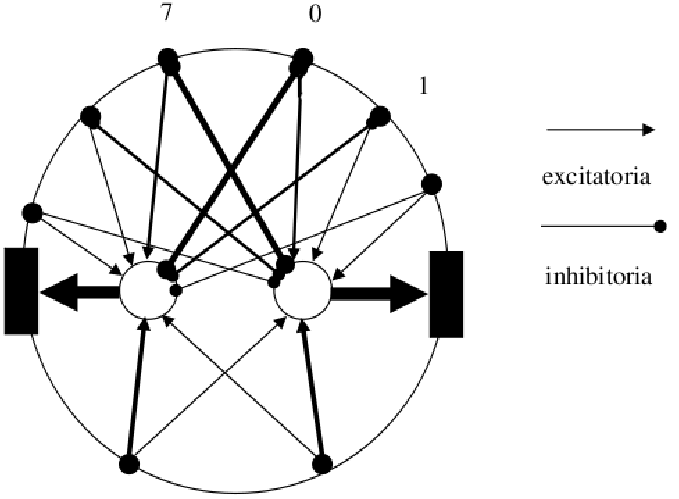
\includegraphics[scale=0.4]{comportamientos/figures/red.png}
\caption{Red neuronal entre los sensores de distancia y los motores}
\label{fig:redN}
\end{center}
\end{figure}

\subsubsection{Salir de situaciones no deseadas}
\label{out_of_unwanted_situations}
\emph{Salir de situaciones no deseadas} surgi\'o como un comportamiento
para ayudar al objetivo de crear un robot aut\'onomo. Con las sucesivas
simulaciones observamos que hab\'ia situaciones donde corr\'ia
peligro la autonom\'ia del robot. Un ejemplo de estas situaciones es el caso
donde dos comportamientos se ``activan mutuamente''.
\\\indent
Para ver esto m\'as claramente, supongamos dos comportamientos $A$ y $B$ con
nivel en la jerarqu\'ia $N(A)$ y $N(B)$, siendo $N(A) > N(B)$. Si la respuesta
a un est\'imulo de $A$ lleva a la activaci\'on de $B$ y a la desactivaci\'on de
$A$ y luego la respuesta de $B$ lleva a la activaci\'on de $A$, podr\'ia llegar
a entrarse en un ciclo si es que esta situaci\'on se da por un tiempo
prolongado o indeterminado. El mayor peligro para la autonom\'ia ocurre
cuando $A$ es el comportamiento de \emph{evitar obst\'aculos} y $B$ es el
comportamiento de \emph{ir a zona de recarga de bater\'ia} ya que el robot
podr\'ia terminar qued\'andose sin bater\'ia en ese ciclo.

\paragraph{Detalle del comportamiento}
Las situaciones no deseadas se dan la mayor\'ia de los casos cuando un
comportamiento hace girar al robot hacia un lado y el otro comportamiento hacia
el lado contrario, aproximadamente en la misma magnitud. \'Esto quiere decir
que la posici\'on del robot se mantiene alrededor de un punto por un per\'iodo
prolongado de tiempo, por lo que decidimos tomar este hecho como est\'imulo
para la activaci\'on de este comportamiento.
\\\indent
La respuesta del comportamiento es, girar un \'angulo que cambie la
direcci\'on del robot y adem\'as que la suma de ese \'angulo repetidas veces no
sea peri\'odica o lo sea luego de una gran cantidad de giros como por ejemplo,
un valor de $\frac{\pi}{4}+0.1$.
Esta \'ultima condici\'on se pide por el siguiente escenario:
\begin{itemize}
	\item Los comportamientos $A$ y $B$ se ``activan mutuamente'' cuando la
		orientaci\'on del robot es $0$.
	\item Los comportamientos $C$ y $D$ se ``activan mutuamente'' cuando la
		orientaci\'on del robot es $\pi$.
	\item La respuesta de \emph{salir de situaciones no deseadas} es girar un
		\'angulo $\pi$.
\end{itemize}

\paragraph{Implementaci\'on del comportamiento}
\begin{verbatim}
    angulo_actual = obtener_angulo_actual(odometria)
    nuevo_angulo = angulo_actual + ANGULO_A_SUMAR
    girar(nuevo_angulo)
\end{verbatim}

